\section{Summary}
We have here shown that the future of companies can be predicted from their interaction networks, even in the absence of any other financial information. Previous works have shown that the topological information of this network combined with label propagation can be used to predict the future success or collapse of a network. We have shown that using GCN outperforms existing methods, as has been shown in many other graph machine learning domains \cite{kipf2016semi}. In the presence of multiple graphs, a single GCN is slightly better than a GCN for each graph, probably since the relation between the graph and the companies' success changes only slowly over time. However, when the same combined network is solved using an LSTM GCN, the performance is significantly increased, suggesting that while the dynamics of companies may change slowly, capturing the dynamics of the change allows the information from previous years to significantly improve on the accuracy of future years, especially following crises. The current formalism can be extended to any multi-network classification tasks, where the networks and tags change slowly enough.

\begin{figure}[h!]
    \begin{center}
         \subfigure[company network]{\label{fig:auc_models_a}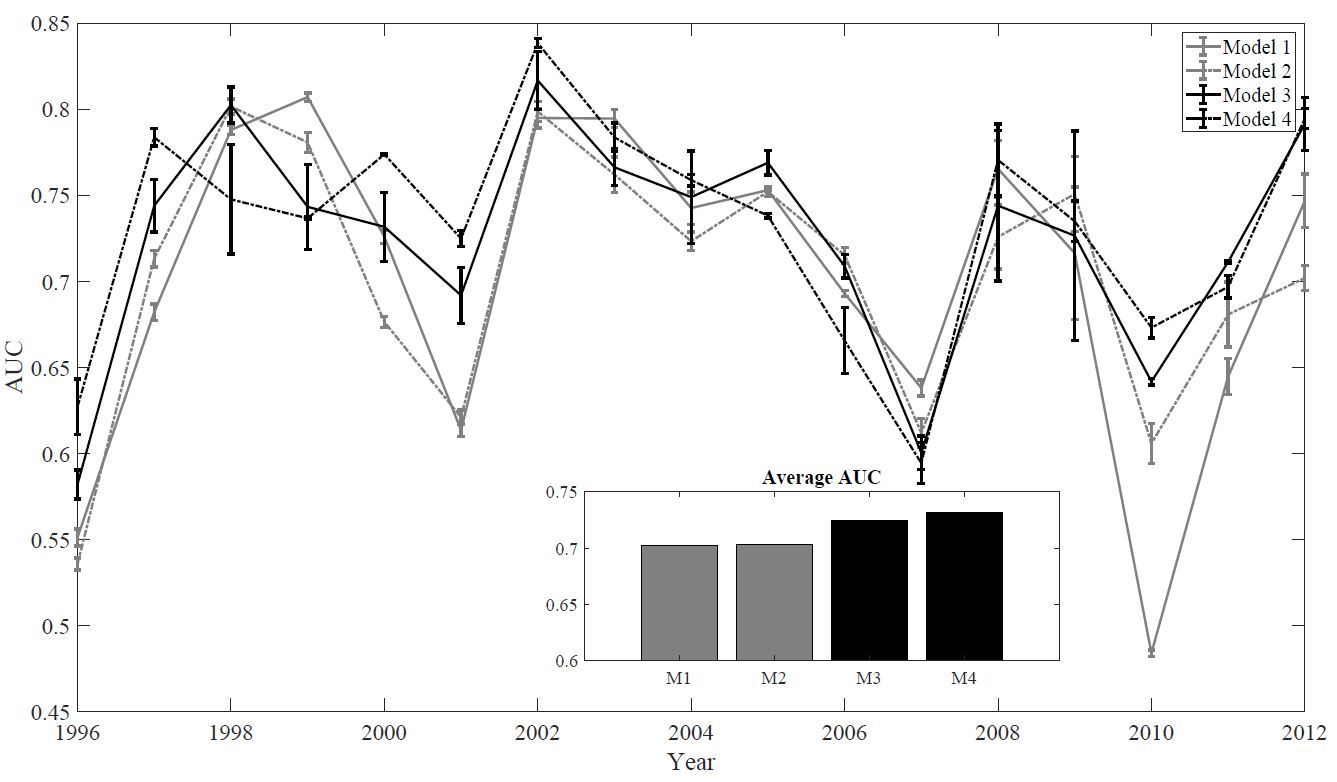
\includegraphics[width=\textwidth]{auc_models_a}}
         \subfigure[blog network]{\label{fig:auc_models_b}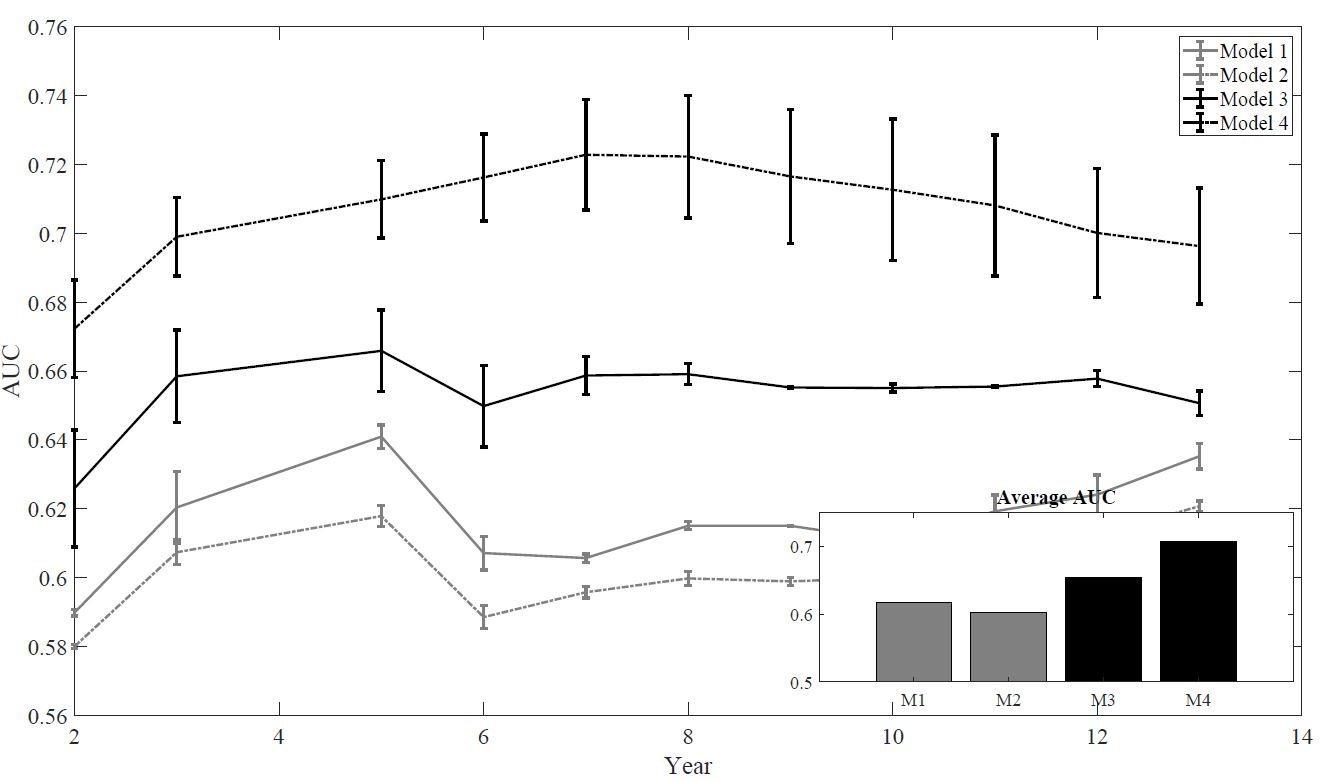
\includegraphics[width=\textwidth]{auc_models_b}}
    \end{center}
    \caption{\textit{Test AUC of the 4 models over the years and average (inset). We have here used only the best input type in the first model for consistency. The results with other input types all show the same ordering, but with lower accuracy.}}
    \label{fig:auc_models}
\end{figure}
